\documentclass[]{subfiles}

\begin{document}
    \marginnote{\textbf{\textit{VL 4}}\\17.04.2023, 11:45}[-1cm]
    \subsection{Der elektrische Aufbau der Atome, das Elektron}
        \subsubsection*{Entdeckung der Kanalstrahlen, Ionen}
            Der Physiker E. Goldstein (~1886) entdeckte die sogenannten \href{https://de.wikipedia.org/wiki/Kanalstrahlen}{\emph{Kanalstrahlen}}, neuer genannt auch \href{https://de.wikipedia.org/w/index.php?title=Ionenstrahlung&redirect=no}{Ionenstrahlung}. Sie dienen der Untersuchung der Gasentladung. Die Funktionsweise der Kanalstrahlen ist wie folgt:
            Die Ionen werden per elektrischem Feld beschleunigt und zur Kathode gelenkt. Sie treten durch die Löcher (auch Defektelektronen) in der Kathode aufgrund ihrer Massenträgheit hindurch, was in Form von Leuchterscheinungen erkennbar ist. 
            Man kann durch dieses Verfahren auf das Verhältnis $e/m$ schließen. 

        \subsubsection*{Entdeckung der Kathodenstrahlen, Elektronen}\label{Ub:Kathodenstrahl}\marginnote{$\to$ \hyperref[Ub:AtomEigenschaften]{\faBook}}
            Über eine Weiterentwicklung der Vakkuumtechnologie im Allgemeinen wird es möglich, sogar Elektronenstrahlen zu erzeugen. Dies geschieht in der sogenannten \href{https://de.wikipedia.org/wiki/Kathodenstrahlröhre}{\textit{Kathodenstrahlröhre}}:
            \begin{figure}[H]
                \centering
                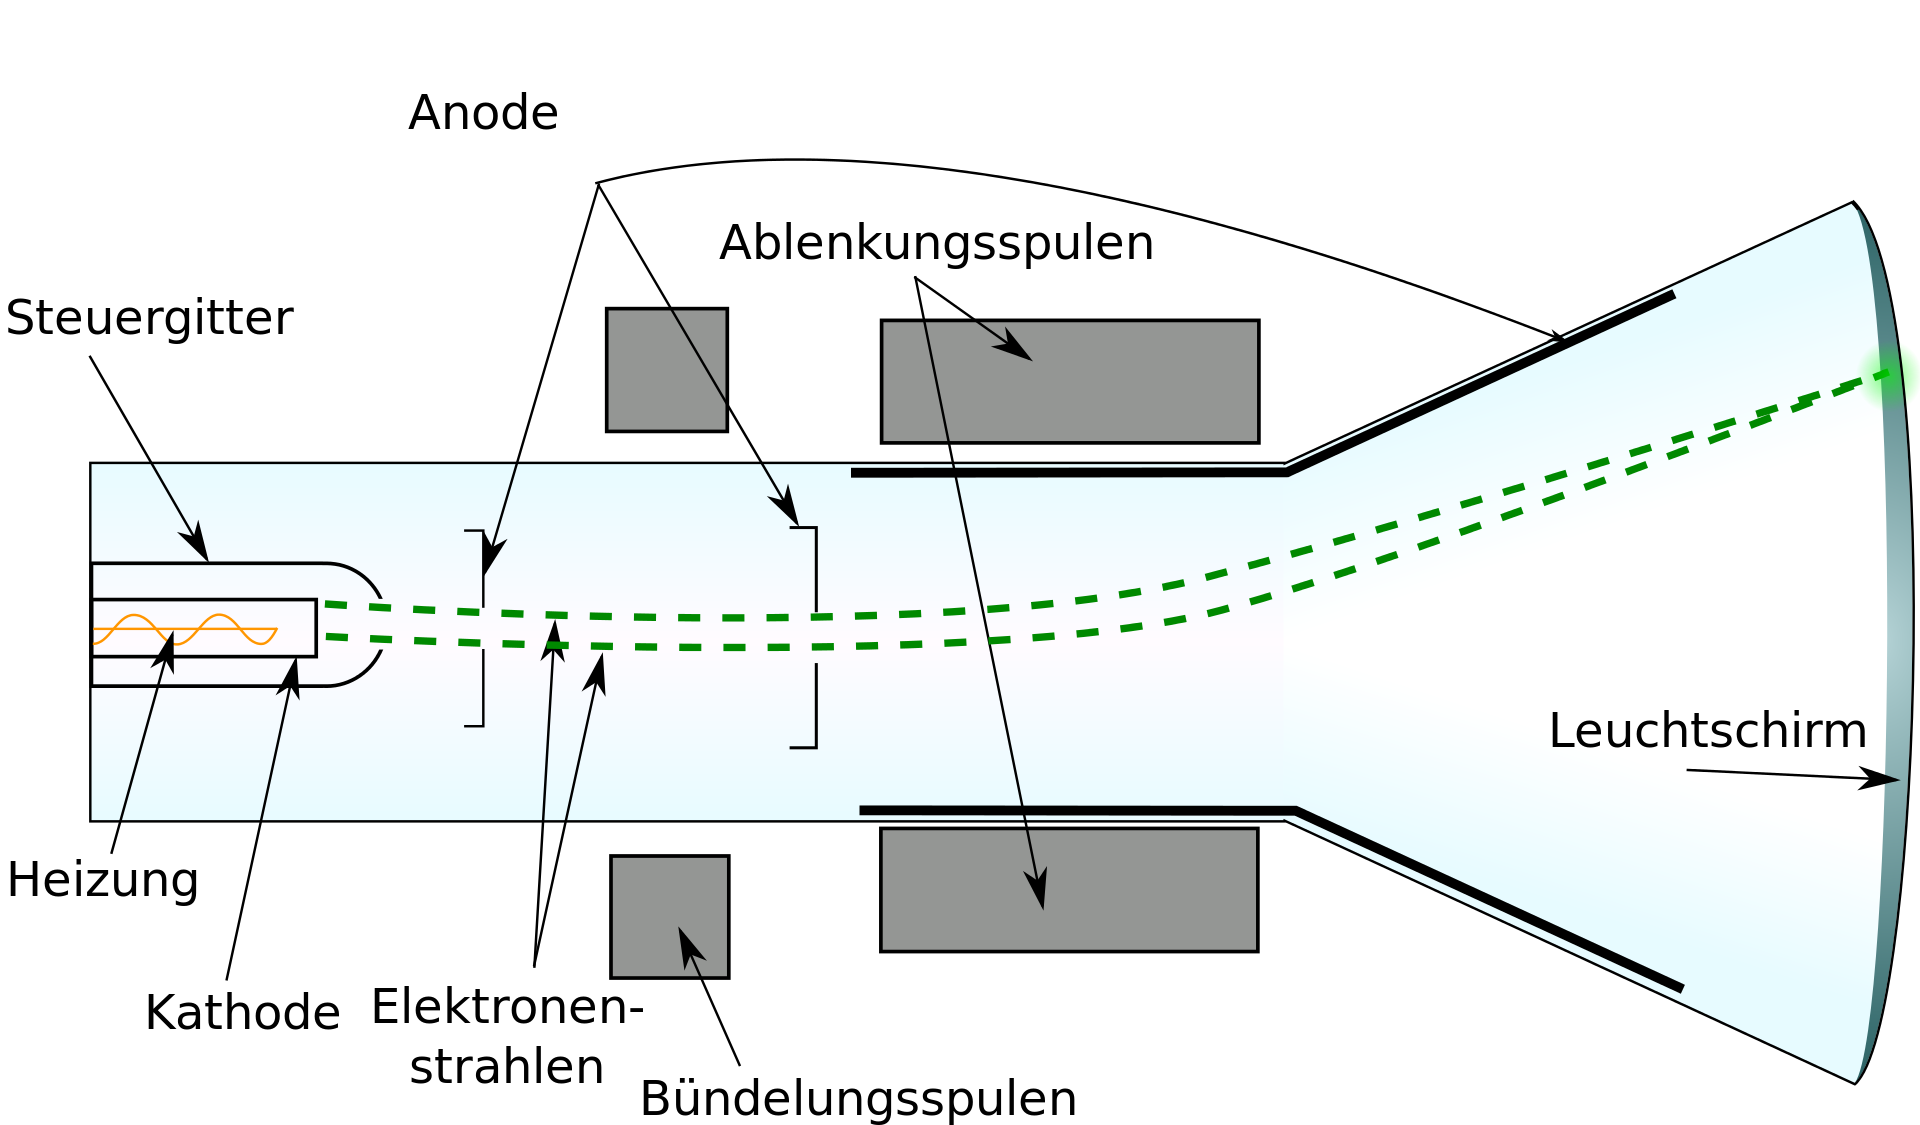
\includegraphics[width=5cm]{Bilddateien/Kathodenstrahlroehre.png}
                \caption{Schematischer Aufbau der Kathodenstrahlröhre.}
            \end{figure}
            [$\to$ Live-Versuch] Es findet nach der Erzeugung des Elektronenstrahls also eine Ablenkung desselben durch ein elektromagnetisches Feld vor. Die Versuche gehen auf den Physiker J. J. Thomson zurück, welcher 1897 die erste Kathodenstrahlröhre baute. 
            Das Massenverhältnis $m_e/m_p$ lautet in diesem Fall 
            \[\frac{m_{Ion}}{e}\approx 10^{-4}.\]
            \begin{Aufgabe}
                \nr{} Suche nach einer Formel zur konkreten Berechnung auf Grundlage der Versuchsbedingungen.
            \end{Aufgabe}
            
        \subsubsection*{Masse des Elektrons}
            Die Bestimmung von $m_e$ aus den massenspektrometrischen Experimenten erfolgt bei bekannter Ladung durch die einfache Multiplikation $m_e/e\cdot e=m_e$. Der Literaturwert der Elektronenladung ist $e=1,602\cdot 10^{-19}\si\coulomb$, die Masse des Elektrons ist $m_e=9,109\cdot 10^{-31}\si{\kilo\gramm}$. 

        \subsubsection*{Ladung des Elektrons (Elementarladung)}\label{Ub:Millikan}\marginnote{$\to$ \hyperref[Ub:AtomEigenschaften]{\faBook}}
            Von Robert Millikan (1909) wurde ein Experimentvorschlag der Elementarladungsbestimmung vorgeschlagen, das sogenannte \href{https://de.wikipedia.org/wiki/Millikan-Experiment}{Millikan-Experiment} [$\to$ AP3]. Ziel des Experimentes ist mithilfe der Annahme eines Kugelvolumens die Masse des Tröpfchens, welche durch Kraftberücksichtigung von Schwerkraft $F_g=m\cdot g$, der Reibung $F_R = 6\pi \cdot \eta \cdot r \cdot v$ und der Auftriebskraft $F_A = V\cdot \rho\cdot g$ indirekt durch den Teilchenradius 
            \[r = \nbra{\frac{9\cdot\eta\cdot v}{2\cdot g\cdot (\rho_\textit{Öl} - \rho_\textit{Luft})}}^{\frac{1}{2}}\implies m=\frac{4}{3}\pi r^3\cdot \rho_\textit{Öl}\tag{\star}\]
            bestimmbar wird. Die Spannung zwischen den Kondensatorplatten liefert die Feldstärke $E=U/d$, welche genau so justiert wird, daß das Teilchen zu schweben beginnt. Das Kräftegleichgewicht liefert dann das Ergebnis
            \[n\cdot e = \frac{\frac{4}{3}\pi r^3\cdot g\cdot \nbra{\rho_\textit{Öl} - \rho_\textit{Luft}}}{E}.\tag{\star}\]
            Hinzukommende Röntgenstrahlung ändert nun schließlich die Tröpfchenladung in Stufen $\Delta q=n\cdot e$, wodurch die Existenz der Elementarladung $e$ bewiesen werden kann [$\to$ \href{https://de.wikipedia.org/wiki/Ionisierende_Strahlung}{Ionisierende Strahlung}]. 
            \begin{Aufgabe}
                \nr{} Führe die angedeutete Rechnung konkret durch. 
            \end{Aufgabe}

        \subsubsection*{Weitere Eigenschaften des Elektrons}\label{Ub:WeitEigElektron}\marginnote{$\to$ \hyperref[Ub:AtomEigenschaften]{\faBook}}
            \paragraph*{Der Eigendrehimpuls (Spin).} Der \href{https://de.wikipedia.org/wiki/Spin}{Spin} kommt in Größen von $\hbar/2$ vor. Er ist ein Quantenzustand, der sich nicht addieren läßt. Nach dem \href{https://de.wikipedia.org/wiki/Standardmodell_der_Teilchenphysik}{\emph{Elementarteilchenmodell}} sind Elektronen Teil der Gruppe \emph{Fermionen}, also Teilchen mit halbzahliger Spinzahl, und in der Untergruppe der \href{https://de.wikipedia.org/wiki/Lepton}{Leptonen}. Teilchen mit ganzzahliger Spinzahl heißen \emph{Bosonen}. 

            \paragraph*{Fermi-Dirac-Statistik.} Die \href{https://de.wikipedia.org/wiki/Fermi-Dirac-Statistik}{\emph{Fermi-Dirac-Statistik}} beschreibt die Wahrscheinlichkeit, daß ein Fermion in einem bestimmten Zustand ist. Sie ist definiert durch 

            \paragraph*{Pauli-Prinzip.} Das \href{https://de.wikipedia.org/wiki/Pauli-Prinzip}{\emph{Pauli-Prinzip}} besagt, daß zwei Fermionen nicht denselben Quantenzustand haben können.

            \paragraph*{Magnetisches Moment.} Ein Elektron weist ein \href{https://de.wikipedia.org/wiki/Magnetisches_Moment}{\emph{Magnetisches Moment}} auf, welches sich aus der Spin-Bewegung ergibt. Es ist definiert durch
            \[\vec{\mu_S} = -g_S\cdot \frac{e}{2\cdot m_e}\cdot\vec{s}.\]

            \begin{Aufgabe}
                \nr{} Recherchiere in einer Mußestunde die genannten Begriffe und versuche, sie zu verstehen.
            \end{Aufgabe}

    \subsection{Bestimmung der Ladungsverteilung im Atom (Streuexperimente)}
        Aus den vorgehenden Kapiteln kann man entnehmen, daß Atomen aus $z\in\N_0$ Elektronen der Ladung $-z\cdot \abs{e}$ und $z$ positiven Ladungen der Ladung $z\cdot\abs{e}$ konstruiert sind. Hieraus resultiert die \emph{elektrische Neutralität} des Atoms. 

        \subsubsection*{Das Thomson'sche Atommodell}\label{Ub:ThomsonAtom}\marginnote{$\to$ \hyperref[Ub:AtomEigenschaften]{\faBook}}
            Das \href{https://de.wikipedia.org/wiki/Thomsonsches_Atommodell}{Thomson'sche Atommodell} (auch Rosinenkuchenmodell) besagt, daß die Ladungen über das gesamte Atomvolumen verteilt sind. Die Ladungsdichte $\rho$ ist also konstant und gleich der Ladung pro Volumeneinheit. 
            \begin{figure}[H]
                \centering
                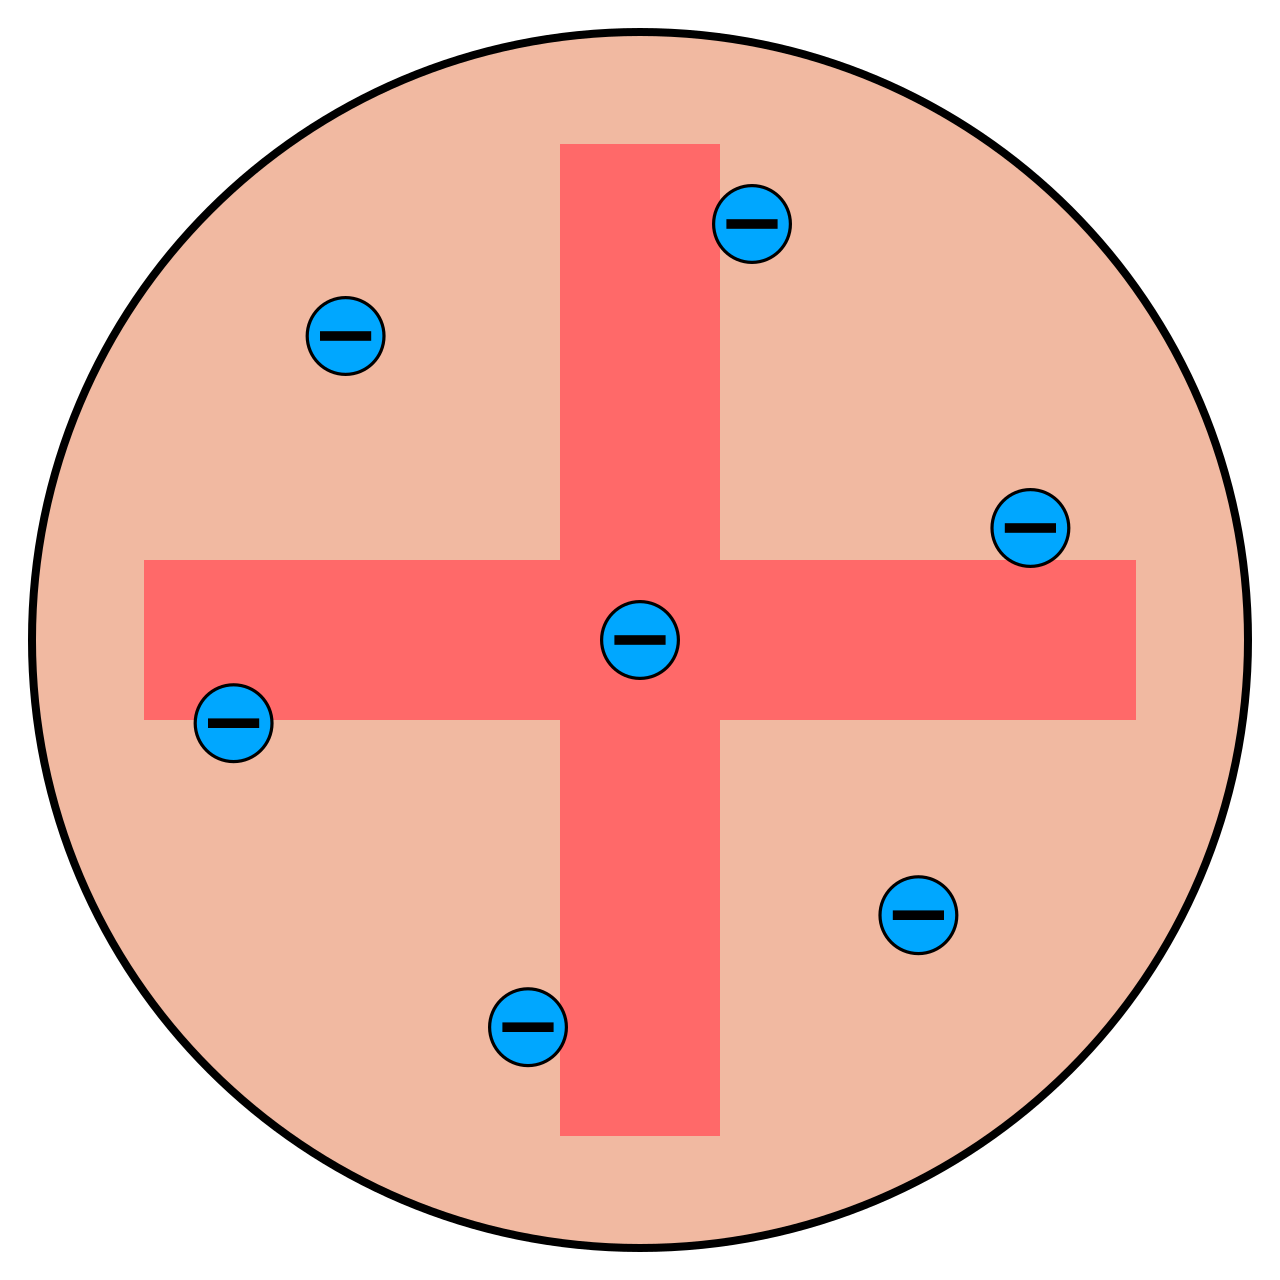
\includegraphics[width=5cm]{Bilddateien/ThomsonModell.png}
                \caption{Das Thomson'sche Atommodell.}
                \label{fig:ThomsonAtom}
            \end{figure}
            Die Bestimmung des inneren Atomaufbaus erfolgt durch die Streuung von $\alpha$ ($_2^4\text{He}^{2+}$) Teilchen und ihrer Bahnanalyse. 

        \subsubsection*{Das Rutherford-Experiment}\label{Ub:RutherfordExp}\marginnote{$\to$ \hyperref[Ub:AtomEigenschaften]{\faBook}}
            Das Experiment entstammt der Idee der drei Physiker E. Marsden, H. Geiger und E. Rutherford. 
            Der Versuchsaufbau ist von der Form 
            \begin{figure}[H]
                \centering
                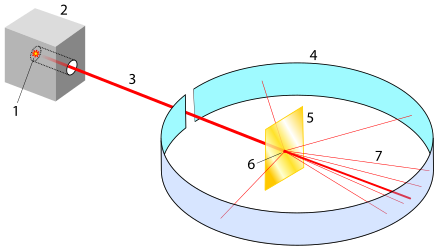
\includegraphics[width=5cm]{Bilddateien/Streuversuch_Rutherford.svg.png}
                \caption{Das Rutherford-Experiment.}
                \label{fig:RutherfordExperiment}
            \end{figure}
            Mit einem \href{https://de.wikipedia.org/wiki/Szintillator}{\emph{Szintillator}} (oder technisch weiter fortgeschrittenen Messgeräten) wird Anzahl der Teilchenregistrierungen in Form von Blitzen in Abhängigkeit des Winkels $\theta$ gemessen, woraus sich zeitlich die Zählrate $N(\theta)$ ergibt. 

            \begin{Aufgabe}
                \nr{} Recherchiere den \emph{Rutherfordschen Streuungsquerschnitt} und versuche, ihn zu verstehen.
            \end{Aufgabe}

            \begin{Experiment}{Rutherford-Experiment}\label{exp:Rutherford}
                Wir führen das Rutherford-Experiment durch und erhalten:
                \begin{table}[H]
                    \centering
                    \begin{tabular}{c|cc|c}
                        Registrierungen & Winkel & Zeit & Folie\\
                        \hline
                        1468\text{cps} & $0\si\degree$ & $20\si\second$ & ohne \\
                        0 \text{cps} & $15\si\degree$ & $20\si\second$ & ohne \\
                        \hline
                        1369 \text{cps} & $0\si\degree$ & $20\si\second$ & mit \\
                        4 \text{cps} & $15\si\degree$ & $20\si\second$ & mit \\
                    \end{tabular}
                    \caption{Vergleich Messung mit und ohne Folie.}
                \end{table}
                (Einheit \href{https://de.wikipedia.org/wiki/Counts_per_second}{\enquote{cps}} ist \emph{counts per second})
            \end{Experiment}

\end{document}